\documentclass{beamer}
\usepackage[utf8]{inputenc}

\usetheme{Madrid}
\usecolortheme{default}
\usepackage{amsmath,amssymb,amsfonts,amsthm}
\usepackage{txfonts}
\usepackage{tkz-euclide}
\usepackage{listings}
\usepackage{adjustbox}
\usepackage{array}
\usepackage{tabularx}
\usepackage{gvv}
\usepackage{lmodern}
\usepackage{circuitikz}
\usepackage{tikz}
\usepackage{graphicx}

\setbeamertemplate{page number in head/foot}[totalframenumber]

\usepackage{tcolorbox}
\tcbuselibrary{minted,breakable,xparse,skins}



\definecolor{bg}{gray}{0.95}
\DeclareTCBListing{mintedbox}{O{}m!O{}}{%
  breakable=true,
  listing engine=minted,
  listing only,
  minted language=#2,
  minted style=default,
  minted options={%
    linenos,
    gobble=0,
    breaklines=true,
    breakafter=,,
    fontsize=\small,
    numbersep=8pt,
    #1},
  boxsep=0pt,
  left skip=0pt,
  right skip=0pt,
  left=25pt,
  right=0pt,
  top=3pt,
  bottom=3pt,
  arc=5pt,
  leftrule=0pt,
  rightrule=0pt,
  bottomrule=2pt,
  toprule=2pt,
  colback=bg,
  colframe=orange!70,
  enhanced,
  overlay={%
    \begin{tcbclipinterior}
    \fill[orange!20!white] (frame.south west) rectangle ([xshift=20pt]frame.north west);
    \end{tcbclipinterior}},
  #3,
}
\lstset{
    language=C,
    basicstyle=\ttfamily\small,
    keywordstyle=\color{blue},
    stringstyle=\color{orange},
    commentstyle=\color{green!60!black},
    numbers=left,
    numberstyle=\tiny\color{gray},
    breaklines=true,
    showstringspaces=false,
}
%------------------------------------------------------------
%This block of code defines the information to appear in the
%Title page
\title %optional
{1.5.18}
\date{August 29,2025}


\author 
{Josyula G S Avaneesh - EE25BTECH11030}



\begin{document}


\frame{\titlepage}
\begin{frame}{Question}
Find the coordinates of a point $\vec{A}$ where $\vec{AB}$ is the diameter of the circle whose center is $\myvec{2\\-3 }$ and $\vec{B}$ is the point $\myvec{1\\4}$.
\end{frame}



\begin{frame}{Theoretical Solution}

Let the vector $\vec{A}$  be required vector to be found

Given,

Circle with Center (say) $\vec{P}$ and
Diameter $\vec{AB}$ 
\begin{align}
    \vec{B}=\myvec{1\\4} \vec{P} = \myvec{2\\-3}
\end{align}

\end{frame}

\begin{frame}{Equation}

\textbf{Center of a circle is the mid point of the diameter. For a circle with center $\vec{P}$ and ends of diameters represented by vectors $\vec{A}$ and $\vec{B}$  }
\begin{align}
    \vec{P}=\frac{\vec{A}+\vec{B}}{2}
\end{align}

\end{frame}

\begin{frame}{Theoretical Solution}

To find vector $\vec{A}$ , we know that $\vec{P}$ divides diameter $\vec{AB}$ in ratio $1\colon1$
\begin{align}
    \therefore \vec{P} = \frac{\vec{A} + \myvec{1\\4}  }{2} 
\end{align}
\begin{align}
    \myvec{2\\-3} = \frac{\vec{A} + \myvec{1\\4}}{2}    
\end{align}

\end{frame}

\begin{frame}{Theoretical Solution}
Rearranging the terms , we get  
\begin{align}
    \vec{A} = \myvec{4-1\\-6-4} 
\end{align}
Hence , 
\begin{align}
    \vec{A} = \myvec{3\\-10}
\end{align}

\end{frame}

\begin{frame}[fragile]
    \frametitle{C Code (1) - Function to find A matrix }

    \begin{lstlisting}

#include <stdio.h>
#include <math.h>
void func(double *P, double *B, double *A , int m )
{
    for ( int i = 0 ; i < m ; i++ )
    {
        A[i] = 2*P[i] - B[i] ; 
    }

}
    \end{lstlisting}
\end{frame}
\begin{frame}[fragile]
    \frametitle{C Code (1) - Function to Find Radius}

    \begin{lstlisting}

double radius(double *P , double *B , int m )
{
    double sum = 0.0; 
    for ( int i = 0 ; i < m ; i++ )
    {
        sum += pow(P[i]-B[i] , 2 );
    }
    return sqrt(sum) ; 
}

    \end{lstlisting}
\end{frame}


\begin{frame}[fragile]
    \frametitle{C Code (2) - Function to Generate Points on Circle}

    \begin{lstlisting}

#include <math.h>

void circle_gen(double *X , double *Y , double *P, int n , double r)
{
// n is no. of points to generates. x stores x coor , y stores y coor 
    for (int i  = 0 ; i < n ; i++ )
    {
        double theta = 2.0 * M_PI * i / n ; 
        X[i] = P[0] + r * cos(theta);
        Y[i] = P[1] + r * sin (theta); 
    }   
}
    \end{lstlisting}
\end{frame}
\begin{frame}[fragile]
    \frametitle{C Code (2) - Function to Generate Points on Line}

    \begin{lstlisting}
void line_gen (double *X, double *Y , double *A , double *B , int n , int m )
{
    double temp[m] ; 
    for (int i = 0 ; i < m ; i++)
    {
        temp [ i ] = (B[i]- A[i]) /(double) n ; 
    }
    for (int i = 0 ; i <= n ; i++ )
    {
        X[i] = A[0] + temp[0] * i ; 
        Y[i] = A[1] + temp[1] * i ;
    }
}



    \end{lstlisting}
\end{frame}

\begin{frame}[fragile]
    \frametitle{Python Code - Using Shared Object}
    \begin{lstlisting}

import ctypes
import numpy as np
import matplotlib.pyplot as plt

handc1 = ctypes.CDLL("./functions.so")

handc1.func.argtypes = [
    ctypes.POINTER(ctypes.c_double),
    ctypes.POINTER(ctypes.c_double),
    ctypes.POINTER(ctypes.c_double),
    ctypes.c_int
]
handc1.func.restype = None # void function
\end{lstlisting}
\end{frame}

\begin{frame}[fragile]
    \frametitle{Python Code - Using Shared Object}
    \begin{lstlisting}
m = 2

P = np.array([[2],[-3]], dtype=np.float64)
B = np.array([[1],[4]], dtype=np.float64)
A = np.zeros(m, dtype=np.float64)

handc1.func(
    P.ctypes.data_as(ctypes.POINTER(ctypes.c_double)),
    B.ctypes.data_as(ctypes.POINTER(ctypes.c_double)),
    A.ctypes.data_as(ctypes.POINTER(ctypes.c_double)),
    m #len(P) alternate
)
\end{lstlisting}
\end{frame}

\begin{frame}[fragile]
    \frametitle{Python Code - Using Shared Object}
    \begin{lstlisting}

handc1.radius.argtypes = [
    ctypes.POINTER(ctypes.c_double),
    ctypes.POINTER(ctypes.c_double),
    ctypes.c_int
]

handc1.radius.restype = ctypes.c_double #return double

radius = handc1.radius(
    P.ctypes.data_as(ctypes.POINTER(ctypes.c_double)),
    B.ctypes.data_as(ctypes.POINTER(ctypes.c_double)),
    m
)
\end{lstlisting}
\end{frame}

\begin{frame}[fragile]
    \frametitle{Python Code - Using Shared Object}
    \begin{lstlisting}
handc2 = ctypes.CDLL("./circle_line.so")
handc2.line_gen.argtypes = [
    ctypes.POINTER(ctypes.c_double),
    ctypes.POINTER(ctypes.c_double),
    ctypes.POINTER(ctypes.c_double),
    ctypes.POINTER(ctypes.c_double),
    ctypes.c_int,
    ctypes.c_int
]
handc2.line_gen.restype = None
n = 20,m = 2
X_l = np.zeros(n,dtype=np.float64)
Y_l = np.zeros(n,dtype=np.float64)
\end{lstlisting}
\end{frame}

\begin{frame}[fragile]
    \frametitle{Python Code - Using Shared Object}
    \begin{lstlisting}
handc2.line_gen(
    X_l.ctypes.data_as(ctypes.POINTER(ctypes.c_double)),
    Y_l.ctypes.data_as(ctypes.POINTER(ctypes.c_double)),
    A.ctypes.data_as(ctypes.POINTER(ctypes.c_double)),
    B.ctypes.data_as(ctypes.POINTER(ctypes.c_double)),
    n,m)
    
plt.figure()

#plotting line
plt.plot([X_l[0],X_l[-1]],[Y_l[0],Y_l[-1]],"g--",label="Diameter")
plt.scatter(A[0],A[1],color = "red",s=50)
plt.scatter(B[0],B[1],color = "red",s=50)
plt.scatter(P[0],P[1],color = "red",s=50,label = "Center of Circle")
\end{lstlisting}
\end{frame}

\begin{frame}[fragile]
    \frametitle{Python Code - Using Shared Object}
    \begin{lstlisting}
handc2.circle_gen.argtypes = [
    ctypes.POINTER(ctypes.c_double),
    ctypes.POINTER(ctypes.c_double),
    ctypes.POINTER(ctypes.c_double),
    ctypes.c_int,
    ctypes.c_double]

handc2.circle_gen.restypes = None

n = 200
#r = radius 

X_c =  np.zeros(n,dtype=np.float64)
Y_c =  np.zeros(n,dtype=np.float64)
\end{lstlisting}
\end{frame}

\begin{frame}[fragile]
    \frametitle{Python Code - Using Shared Object}
    \begin{lstlisting}

handc2.circle_gen(

    X_c.ctypes.data_as(ctypes.POINTER(ctypes.c_double)),
    Y_c.ctypes.data_as(ctypes.POINTER(ctypes.c_double)),
    P.ctypes.data_as(ctypes.POINTER(ctypes.c_double)),
    n , radius
)

#plotting circle
plt.plot(X_c,Y_c , "b-")

plt.annotate(f"A({A[0]},{A[1]})", (A[0], A[1]), textcoords="offset points", xytext=(0,5), ha='right')
plt.annotate("B", (B[0], B[1]), textcoords="offset points", xytext=(0,5), ha='left')
plt.annotate("P", (P[0], P[1]), textcoords="offset points", xytext=(0,5), ha='left')
\end{lstlisting}
\end{frame}

\begin{frame}[fragile]
    \frametitle{Python Code - Using Shared Object}
    \begin{lstlisting}
# Equal scaling for axes (important for circles!)
plt.gca().set_aspect("equal", adjustable="box")

plt.xlim([-10,10])
plt.ylim([-10,10])

# Labels and title
plt.xlabel("X")
plt.ylabel("Y")
plt.title("1.5.18")

plt.legend(loc = 'upper right')
plt.grid(True)

plt.savefig('figs/circle_graph.png')
subprocess.run(shlex.split("termux-open figs/circle_graph.png"))

    \end{lstlisting}
\end{frame}

\begin{frame}{Plot-Using Both C and Python}
    \centering
    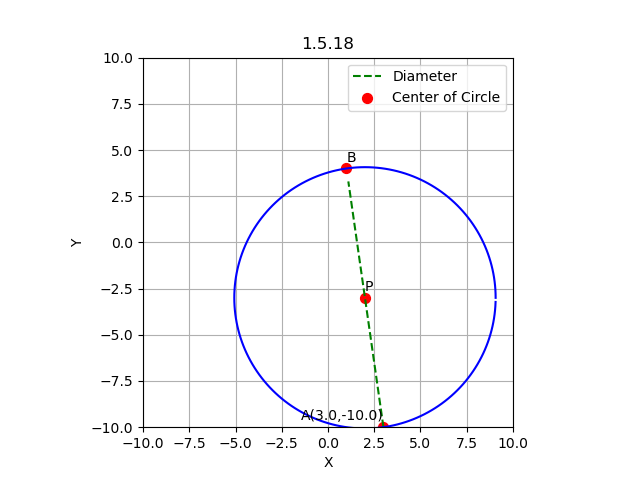
\includegraphics[width=\columnwidth, height=0.8\textheight, keepaspectratio]{figs/circle_graph.png}     
\end{frame}

\begin{frame}[fragile]
    \frametitle{Python Code}
    \begin{lstlisting}
import math
import sys
import numpy as np
import numpy.linalg as LA
import matplotlib.pyplot as plt
import matplotlib.image as mpimg

#local imports
from libs.line.funcs import *
from libs.triangle.funcs import *
from libs.conics.funcs import circ_gen

#if using termux
import subprocess
import shlex
\end{lstlisting}
\end{frame}

\begin{frame}[fragile]
    \frametitle{Python Code}
    \begin{lstlisting}
def func(P, B):
    # NumPy automatically applies operations to each element in the array
    return 2*P -B

def func_radius(P,B) :
    return LA.norm(P-B)

P = np.array([2,-3]).reshape(-1,1)
B = np.array([1,4]).reshape(-1,1)

A = func(P,B).reshape(-1,1)

x_AB = line_gen_num(A,B,20)
radius = func_radius(P,B)


\end{lstlisting}
\end{frame}

\begin{frame}[fragile]
    \frametitle{Python Code}
    \begin{lstlisting}
    x_circ = circ_gen(P,radius)
plt.plot(x_circ[0,:],x_circ[1,:],"red",label="Circle")
plt.plot(x_AB[0,:],x_AB[1,:],"g--",label="Diameter")

tri_coords = np.block([[A,B,P]])
plt.scatter(tri_coords[0,:], tri_coords[1,:])
vert_labels = ['A','B','P']
for i , txt in enumerate(vert_labels):
    plt.annotate(txt,(tri_coords[0,i],tri_coords[1,i]),textcoords="offset points", xytext=(0,10),ha='center')
\end{lstlisting}
\end{frame}

\begin{frame}[fragile]
    \frametitle{Python Code }
    \begin{lstlisting}
plt.xlabel('$x$')
plt.ylabel('$y$')
plt.legend(loc='best')
plt.grid() # minor
plt.axis('equal')
#plt.savefig("../figs/circle_graph2.png")
#plt.show()

plt.savefig('/figs/circle_graph2.png')
subprocess.run(shlex.split("termux-open figs/circle_graph2.png"))


    \end{lstlisting}
\end{frame}


\begin{frame}{Plot-Using only Python}
    \centering
    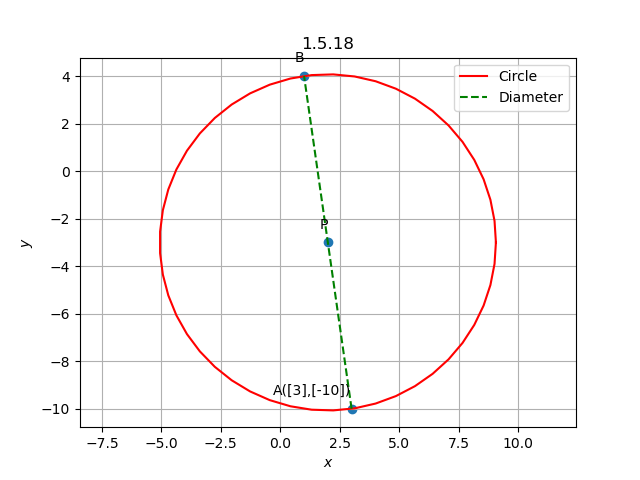
\includegraphics[width=\columnwidth, height=0.8\textheight, keepaspectratio]{figs/circle_graph2.png}     
\end{frame}


\end{document}
